% !TEX root = ../main.tex
\begin{tikzpicture}[line width=1pt,node distance=14mm ,main/.style = {draw, rectangle},scale=1] 
   
   \node[scale=.8] at (7,5.5){$\textup{PerfMatch}[b,\{x_1,x_2\}]$};
       \node[main] at (7,4) (9) {
   \begin{tikzpicture}[line width=1pt,node distance=14mm ,main/.style = {draw, circle},scale=1] 
   \node[main,fill=red!40!white,densely dashed] at (0,1) (x1) {\texttt{$x_1$}};
   \node[main,fill=red!40!white,densely dashed] at (1,1) (x2) {\texttt{$x_2$}};
       \node[main,color=black] at (0,0) (x3) {\texttt{$x_3$}};
       \node[main,color=black] at (1,0) (x4) {\texttt{$x_4$}};
      \draw (x1) -- (x2);
       \draw (x1) -- (x3);
      \draw (x2) -- (x3);
      \draw (x3) -- (x4);
   \end{tikzpicture}
       };
       
   
    \node[scale=.8] at (7,1.5){$\textup{PerfMatch}[c,\{x_2\}]$};
   \node[main] at (7,0) (8) {
   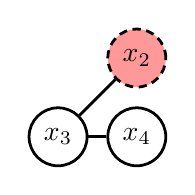
\begin{tikzpicture}[line width=1pt,node distance=14mm ,main/.style = {draw, circle},scale=1] 
   \node[main,fill=red!40!white,densely dashed] at (1,1) (x2) {\texttt{$x_2$}};
       \node[main,color=black] at (0,0) (x3) {\texttt{$x_3$}};
       \node[main,color=black] at (1,0) (x4) {\texttt{$x_4$}};
      \draw (x2) -- (x3);
      \draw (x3) -- (x4);
   \end{tikzpicture}
   };
   
       \draw [decorate,decoration={brace,amplitude=10}] (6,2) -- (8,2) node [black,midway,xshift=-0.6cm] {};
   
   
    \node[scale=.8] at (10.5,5.5){$\textup{PerfMatch}[b,\{x_3,x_4\}]$};
       \node[main] at (10.5,4) (9) {
   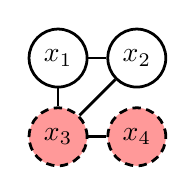
\begin{tikzpicture}[line width=1pt,node distance=14mm ,main/.style = {draw, circle},scale=1] 
   \node[main,color=black] at (0,1) (x1) {\texttt{$x_1$}};
   \node[main,color=black] at (1,1) (x2) {\texttt{$x_2$}};
       \node[main,fill=red!40!white,densely dashed] at (0,0) (x3) {\texttt{$x_3$}};
       \node[main,fill=red!40!white,densely dashed] at (1,0) (x4) {\texttt{$x_4$}};
      \draw (x1) -- (x2);
       \draw (x1) -- (x3);
      \draw (x2) -- (x3);
      \draw (x3) -- (x4);
   \end{tikzpicture}
       };

   
        \draw [decorate,decoration={brace,amplitude=10}] (9.5,2) -- (11.5,2) node [black,midway,xshift=-0.6cm] {};
       \node[scale=0.8] at (10.5,1.5){Cannot form};
       \node[scale=0.8] at (10.5,1.1){a respectful matching};
       %\node[text width=6cm] at (2,-2){$\DP[i,c]$};
       %\node[text width=6cm] at (5.5,-2){$\DP[i,c+\{x_4\to \texttt{gray/dotted}]$};
      
   \end{tikzpicture}
   